\begin{figure}[H]\centering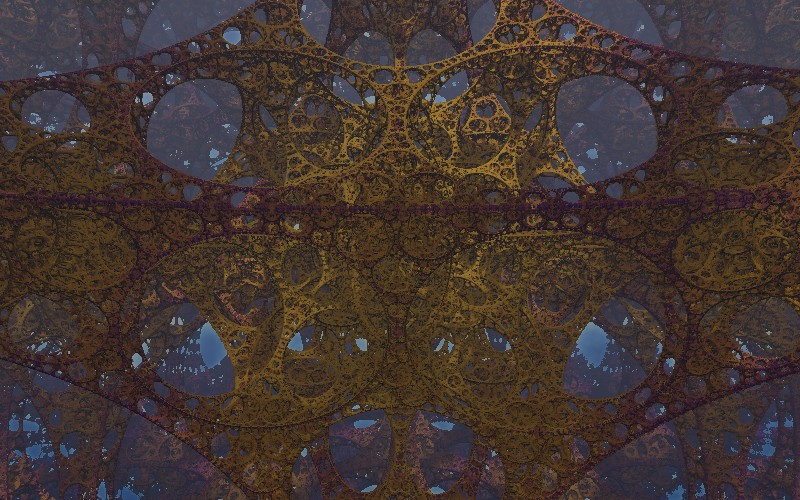
\includegraphics[width=0.88\textwidth]{img/pseudoKleinian.jpg}
\caption{Pseudo-Kleinian, default parameters (9 iterations).}\end{figure}
\paragraph{Parameters (app defaults).} Iterations 9 (range 2--20); step factor 0.8; bounding size 1; \emph{unbounded} (no bounding sphere assumed).

{\footnotesize\begin{tabular}{@{}llrr@{}}\toprule Parameter & Key & Default & Range\\\midrule
Box width & \texttt{boxXY} & 0.908 & 0.4\,\dots\,1.4\\
Box height & \texttt{boxZ} & 0.924 & 0.4\,\dots\,1.6\\
Inversion size & \texttt{size} & 1 & 0.6\,\dots\,1.6\\
Offset X & \texttt{cx} & 0 & $-$0.5\,\dots\,0.5\\
Offset Y & \texttt{cy} & 0 & $-$0.5\,\dots\,0.5\\
Offset Z & \texttt{cz} & 0 & $-$0.5\,\dots\,0.5\\
Thickness & \texttt{thick} & 0.928 & 0.5\,\dots\,1.2\\
\bottomrule\end{tabular}}
